\documentclass[12pt,a4paper]{article}
\usepackage[utf8]{inputenc}
\usepackage[T1]{fontenc}
\usepackage[main=slovak,provide=*]{babel}
\usepackage{tikz}
\usepackage{graphicx}
\usepackage{geometry}
\geometry{margin=2cm}
\pagestyle{empty}

\newcommand{\legendEmptyBox}[2]{%
    \draw[gray, thick] (#1,#2) rectangle ++(0.45,0.45);
}

\newcommand{\legendCrossBox}[2]{%
    \draw[gray, thick] (#1,#2) rectangle ++(0.45,0.45);
    \draw[thick] (#1+0.02,#2+0.02) -- (#1+0.43,#2+0.43);
    \draw[thick] (#1+0.02,#2+0.43) -- (#1+0.43,#2+0.02);
}

\newcommand{\legendCrossOutside}[2]{%
    \draw[gray, thick] (#1,#2) rectangle ++(0.45,0.45);
    \draw[thick] (#1+0.10,#2+0.20) -- (#1+0.50,#2+0.60);
    \draw[thick] (#1+0.10,#2+0.60) -- (#1+0.50,#2+0.20);
}

\newcommand{\legendFilledBox}[2]{%
    \draw[gray, thick] (#1,#2) rectangle ++(0.45,0.45);
    \fill[black!85] (#1,#2) rectangle (#1+0.45,#2+0.45);
}

\newcommand{\legendCircledFilledBox}[2]{%
    \draw[gray, thick] (#1,#2) rectangle ++(0.45,0.45);
    \fill[black!85] (#1,#2) rectangle (#1+0.45,#2+0.45);
    \draw[thick] (#1+0.225,#2+0.225) circle (0.31);
}

\begin{document}

\begin{center}
    {\LARGE\textbf{Legenda k odpovedovým hárkom}}
\end{center}

\vspace{1.5cm}

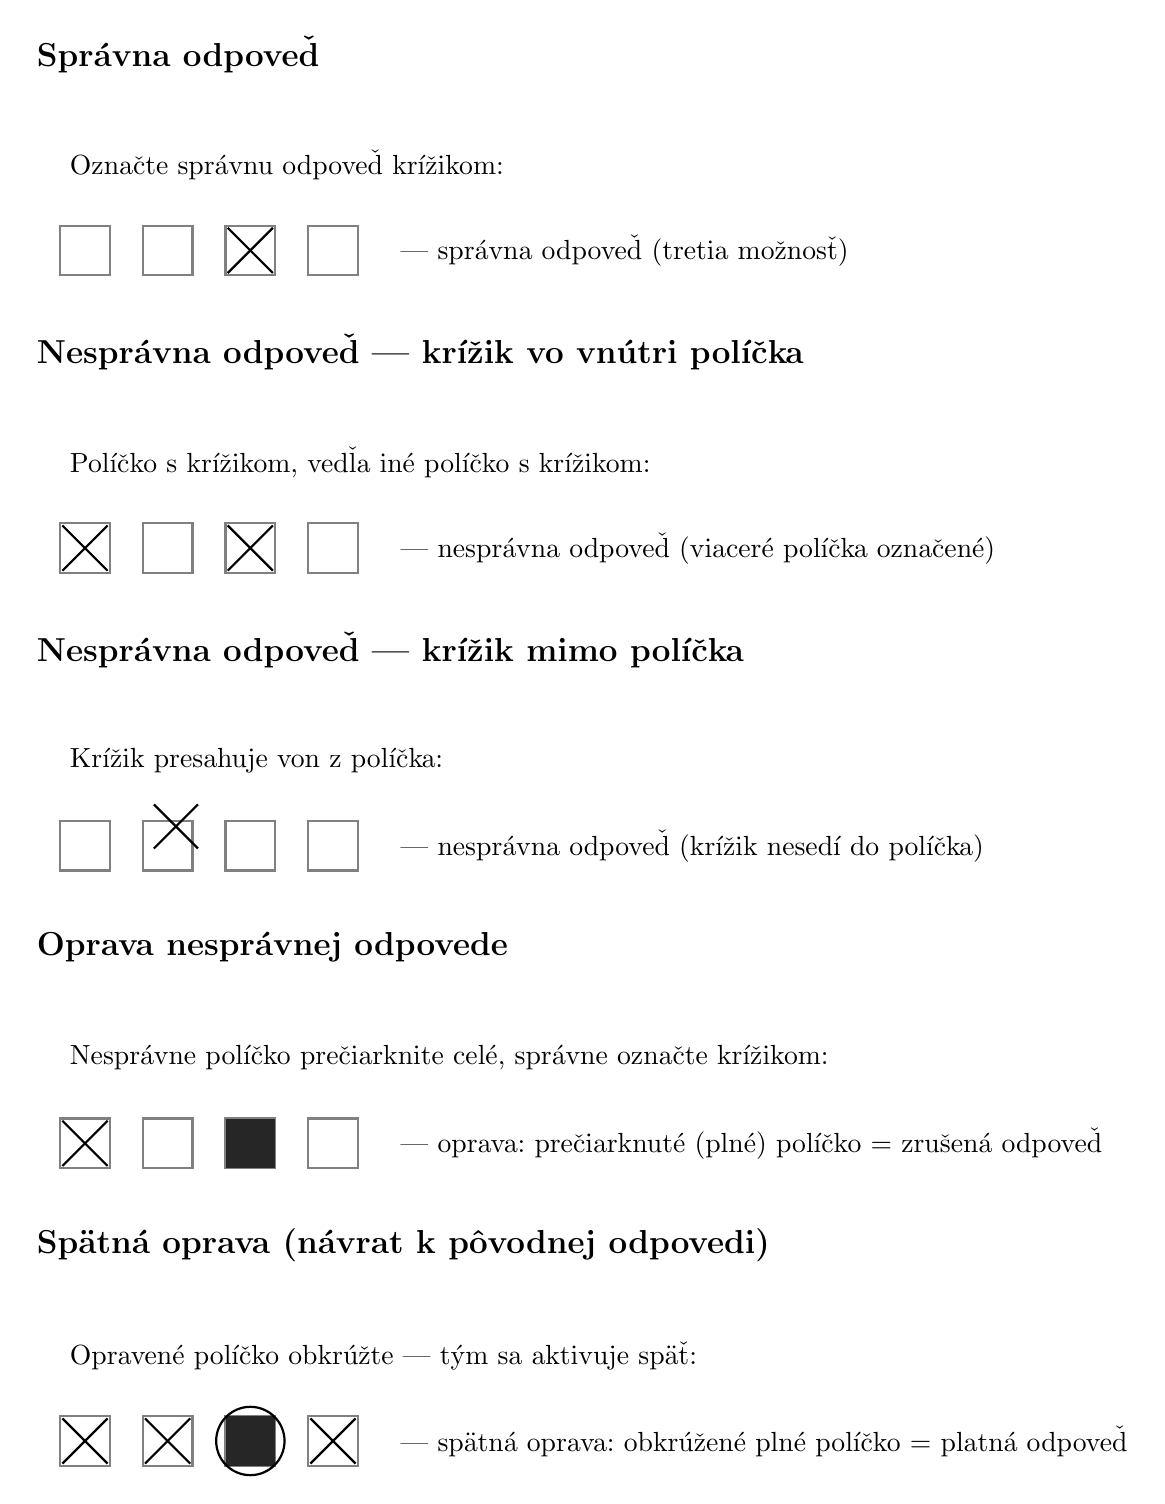
\begin{tikzpicture}[font=\normalsize, scale=1.4]

    % --- ROW 1: Správna odpoveď ---
    \node[anchor=west] at (0, 3.5) {\large\textbf{Správna odpoveď}};
    \node[anchor=west] at (0.3, 2.5) {Označte správnu odpoveď krížikom:};

    \legendEmptyBox{0.3}{1.5}
    \legendEmptyBox{1.05}{1.5}
    \legendCrossBox{1.80}{1.5}
    \legendEmptyBox{2.55}{1.5}

    \node[anchor=west] at (3.3, 1.72) {— správna odpoveď (tretia možnosť)};

    % --- ROW 2: Nesprávna odpoveď (krížik vnútri) ---
    \node[anchor=west] at (0, 0.8) {\large\textbf{Nesprávna odpoveď — krížik vo vnútri políčka}};
    \node[anchor=west] at (0.3, -0.2) {Políčko s krížikom, vedľa iné políčko s krížikom:};

    \legendCrossBox{0.3}{-1.2}
    \legendEmptyBox{1.05}{-1.2}
    \legendCrossBox{1.80}{-1.2}
    \legendEmptyBox{2.55}{-1.2}

    \node[anchor=west] at (3.3, -0.98) {— nesprávna odpoveď (viaceré políčka označené)};

    % --- ROW 3: Nesprávna odpoveď (krížik zvonku) ---
    \node[anchor=west] at (0, -1.9) {\large\textbf{Nesprávna odpoveď — krížik mimo políčka}};
    \node[anchor=west] at (0.3, -2.9) {Krížik presahuje von z políčka:};

    \legendEmptyBox{0.3}{-3.9}
    \legendCrossOutside{1.05}{-3.9}
    \legendEmptyBox{1.80}{-3.9}
    \legendEmptyBox{2.55}{-3.9}

    \node[anchor=west] at (3.3, -3.68) {— nesprávna odpoveď (krížik nesedí do políčka)};

    % --- ROW 4: Oprava ---
    \node[anchor=west] at (0, -4.6) {\large\textbf{Oprava nesprávnej odpovede}};
    \node[anchor=west] at (0.3, -5.6) {Nesprávne políčko prečiarknite celé, správne označte krížikom:};

    \legendCrossBox{0.3}{-6.6}
    \legendEmptyBox{1.05}{-6.6}
    \legendFilledBox{1.80}{-6.6}
    \legendEmptyBox{2.55}{-6.6}

    \node[anchor=west] at (3.3, -6.38) {— oprava: prečiarknuté (plné) políčko = zrušená odpoveď};

    % --- ROW 5: Spätná oprava ---
    \node[anchor=west] at (0, -7.3) {\large\textbf{Spätná oprava (návrat k pôvodnej odpovedi)}};
    \node[anchor=west] at (0.3, -8.3) {Opravené políčko obkrúžte — tým sa aktivuje späť:};

    \legendCrossBox{0.3}{-9.3}
    \legendCrossBox{1.05}{-9.3}
    \legendCircledFilledBox{1.80}{-9.3}
    \legendCrossBox{2.55}{-9.3}

    \node[anchor=west] at (3.3, -9.08) {— spätná oprava: obkrúžené plné políčko = platná odpoveď};

\end{tikzpicture}

\end{document}
